\documentclass{article}
\usepackage{tikz}
\usetikzlibrary{external}
\tikzexternalize[mode=list and make]

\tikzset{
    % Defines a custom style which generates BOTH, .pdf and .png export
    % but prefers the .png on inclusion.
    %
    % This style is not pre-defined, you may need to copy-paste and
    % adjust it.
    png export/.style={
        external/system call/.add={}{; convert -density 300 -transparent white "\image.pdf" "\image.png"},
        %
        /pgf/images/external info,
        /pgf/images/include external/.code={%
            \includegraphics
            [width=\pgfexternalwidth,height=\pgfexternalheight]
            {##1.png}%
        },
    },
    %
    png export,% ACTIVATE
}

\begin{document}

{
% Here we specify the figure will be converted and inserted as PNG
\tikzset{png export}
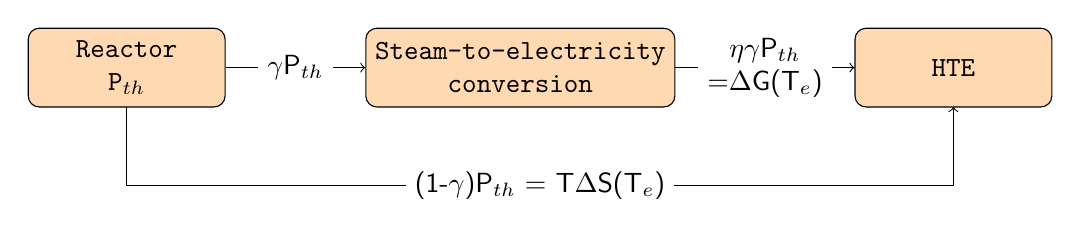
\begin{tikzpicture}[
    base/.style = {rectangle, rounded corners, draw=black,
minimum width=3cm, minimum height=1cm,
text centered, font=\sffamily},
process/.style = {base, minimum width=2.5cm, fill=orange!30,
font=\ttfamily},
node distance=3cm,
every node/.style={fill=white, font=\sffamily}, align=center
]

  \node (reactor) [process] {Reactor\\P$_{th}$};
  \node (steam1)  [process, right of=reactor, xshift=2.cm] {Steam-to-electricity\\conversion};
  \node (hte)     [process, right of=steam1, xshift=2.5cm] {HTE};
  
  \draw[->]     (reactor) -- (steam1) node[midway] {$\gamma$P$_{th}$};
  \draw[->]     (reactor) ++(0.,-0.5)-- ++(0.,-1.)-- node[midway] {(1-$\gamma$)P$_{th}$ = T$\Delta$S(T$_e$)}++(10.5,0.)-- ++(0.,1.);
  \draw[->]     (steam1) -- (hte) node[midway] {$\eta\gamma$P$_{th}$\\ =$\Delta$G(T$_e$)};
\end{tikzpicture}
}

{
\tikzset{png export}
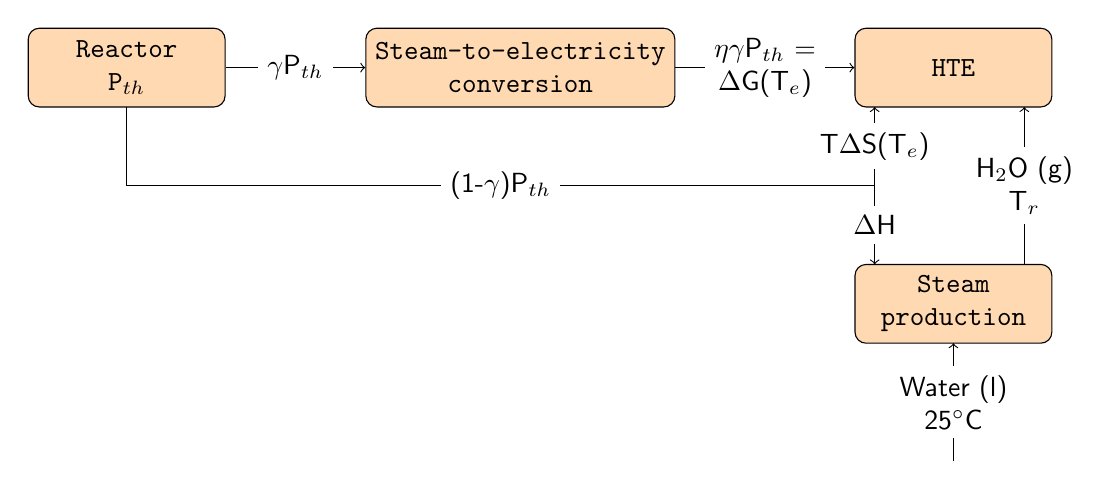
\begin{tikzpicture}[
    base/.style = {rectangle, rounded corners, draw=black,
minimum width=3cm, minimum height=1cm,
text centered, font=\sffamily},
process/.style = {base, minimum width=2.5cm, fill=orange!30,
font=\ttfamily},
node distance=3cm,
every node/.style={fill=white, font=\sffamily}, align=center
]
  % Specification of nodes (position, etc.)

\node (reactor) [process] {Reactor\\P$_{th}$};
\node (steam1)  [process, right of=reactor, xshift=2.cm] {Steam-to-electricity\\conversion};
\node (hte)     [process, right of=steam1, xshift=2.5cm] {HTE};
\node (steam2)  [process, below of=hte, yshift=0.cm, xshift=0.cm] {Steam\\production};

\draw[->]     (reactor) -- (steam1) node[midway] {$\gamma$P$_{th}$};
\draw[->]     (reactor) ++(0.,-0.5)-- ++(0.,-1.)-- node[midway] {(1-$\gamma$)P$_{th}$} ++(9.5,0.)-- node[midway] {T$\Delta$S(T$_e$)} ++(0.,1.);
\draw[->]     (hte) ++(-1,-1.5)-- node[midway] {$\Delta$H} ++(0.,-1.);
\draw[->]     (steam1) -- (hte) node[midway] {$\eta\gamma$P$_{th}$ =\\$\Delta$G(T$_e$)};

\draw[->]     (steam2) ++(0,-2.)-- node[midway] {Water (l)\\25$^\circ$C} ++(0,1.5);
\draw[->]     (steam2) ++(0.9,0.5)-- node[midway] {H$_2$O (g)\\T$_r$} ++(0,2.);

\end{tikzpicture}
}

{
\tikzset{png export}
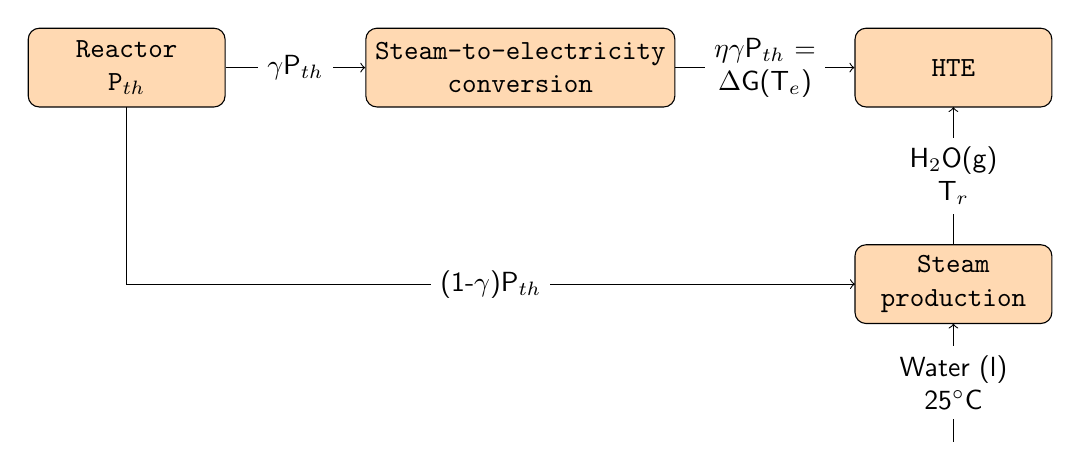
\begin{tikzpicture}[
    base/.style = {rectangle, rounded corners, draw=black,
minimum width=3cm, minimum height=1cm,
text centered, font=\sffamily},
process/.style = {base, minimum width=2.5cm, fill=orange!30,
font=\ttfamily},
node distance=3cm,
every node/.style={fill=white, font=\sffamily}, align=center
]
  % Specification of nodes (position, etc.)

  \node (reactor) [process] {Reactor\\P$_{th}$};
  \node (steam1)  [process, right of=reactor, xshift=2.cm] {Steam-to-electricity\\conversion};
  \node (hte)     [process, right of=steam1, xshift=2.5cm] {HTE};
  \node (steam2)  [process, below of=hte, yshift=0.25cm, xshift=0.cm] {Steam\\production};
  
  \draw[->]     (reactor) -- (steam1) node[midway] {$\gamma$P$_{th}$};
  \draw[->]     (reactor) ++(0.,-0.5)-- ++(0.,-2.25)-- node[midway] {(1-$\gamma$)P$_{th}$} ++(9.25,0.);
  \draw[->]     (steam1) -- (hte) node[midway] {$\eta\gamma$P$_{th}$ =\\ $\Delta$G(T$_e$)};
  
  \draw[->]     (steam2) ++(0,-2.)-- node[midway] {Water (l)\\25$^\circ$C} ++(0,1.5);
  \draw[->]     (steam2) ++(0,0.5)-- node[midway] {H$_2$O(g)\\T$_r$} ++(0,1.75);

\end{tikzpicture}
}

{
\tikzset{png export}
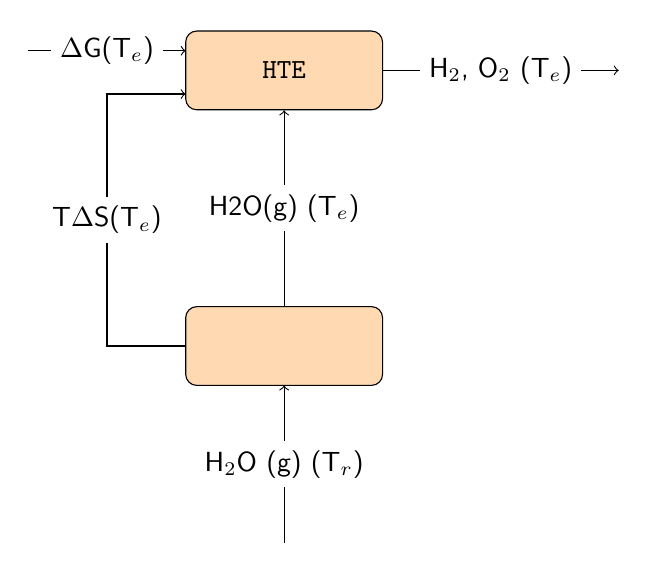
\begin{tikzpicture}[
    base/.style = {rectangle, rounded corners, draw=black,
minimum width=3cm, minimum height=1cm,
text centered, font=\sffamily},
process/.style = {base, minimum width=2.5cm, fill=orange!30,
font=\ttfamily},
node distance=3cm,
every node/.style={fill=white, font=\sffamily}, align=center
]
  % Specification of nodes (position, etc.)

  \node (hte) [process] {HTE};
  \node (split)  [process, below of=hte, yshift=-.5cm] {};
  
  \draw[->]     (hte) ++(-3.25,0.25)-- ++(2,0) node[midway] {$\Delta$G(T$_e$)};
  \draw[->]     (hte) ++(1.25,0)-- ++(3,0) node[midway] {H$_2$, O$_2$ (T$_e$)};
  \draw[->]     (split) -- (hte) node[midway] {H2O(g) (T$_e$)};
  \draw[->]     (split) ++(-1.25,0) -- ++(-1.,0) -- node[midway] {T$\Delta$S(T$_e$)} ++ (0,3.2) -- ++(1.,0);
  \draw[->]     (split) ++(0,-2.5)-- ++(0,2) node[midway] {H$_2$O (g) (T$_r$)};

\end{tikzpicture}
}

{
\tikzset{png export}
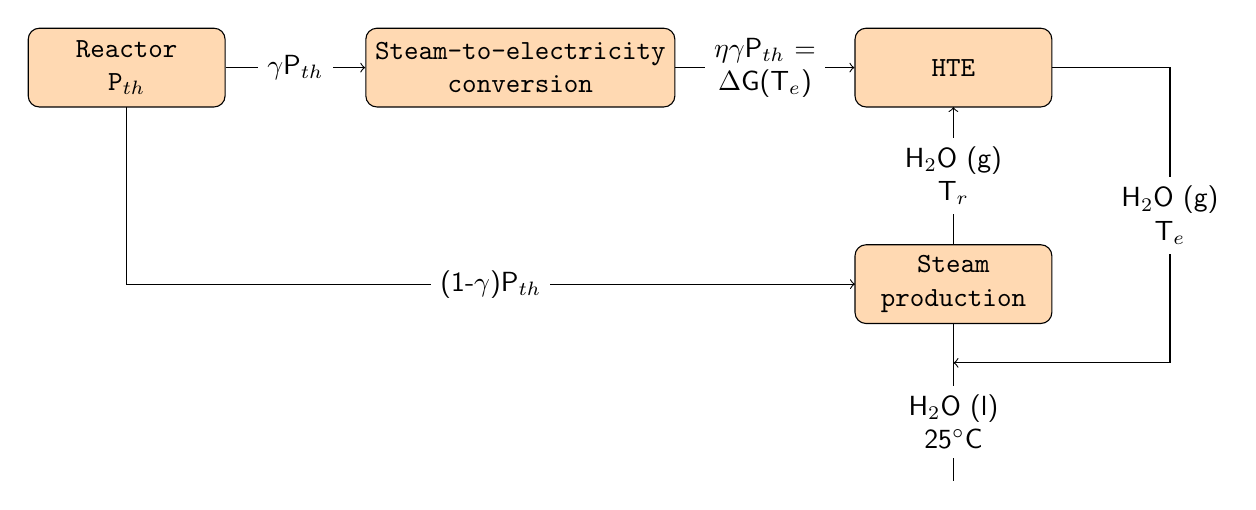
\begin{tikzpicture}[
    base/.style = {rectangle, rounded corners, draw=black,
minimum width=3cm, minimum height=1cm,
text centered, font=\sffamily},
process/.style = {base, minimum width=2.5cm, fill=orange!30,
font=\ttfamily},
node distance=3cm,
every node/.style={fill=white, font=\sffamily}, align=center
]
  % Specification of nodes (position, etc.)

  \node (reactor) [process] {Reactor\\P$_{th}$};
  \node (steam1)  [process, right of=reactor, xshift=2.cm] {Steam-to-electricity\\conversion};
  \node (hte)     [process, right of=steam1, xshift=2.5cm] {HTE};
  \node (steam2)  [process, below of=hte, yshift=0.25cm, xshift=0.cm] {Steam\\production};
  
  \draw[->]     (reactor) -- (steam1) node[midway] {$\gamma$P$_{th}$};
  \draw[->]     (reactor) ++(0.,-0.5)-- ++(0.,-2.25)-- node[midway] {(1-$\gamma$)P$_{th}$} ++(9.25,0.);
  \draw[->]     (steam1) -- (hte) node[midway] {$\eta\gamma$P$_{th}$ =\\ $\Delta$G(T$_e$)};
  
  \draw[-]     (steam2) ++(0,-2.5)-- node[midway] {H$_2$O (l)\\25$^\circ$C} ++(0, 1.5);
  \draw[-]     (steam2) ++(0,-1.)-- ++(0,.5);
  \draw[->]     (steam2) ++(0,0.5)-- node[midway] {H$_2$O (g)\\T$_r$} ++(0,1.75);
  \draw[->]     (hte) ++(1.25, 0)-- ++(1.5, 0)-- node[midway] {H$_2$O (g)\\T$_e$} ++(0, -3.75)-- ++(-2.75, 0);

\end{tikzpicture}
}

{
\tikzset{png export}
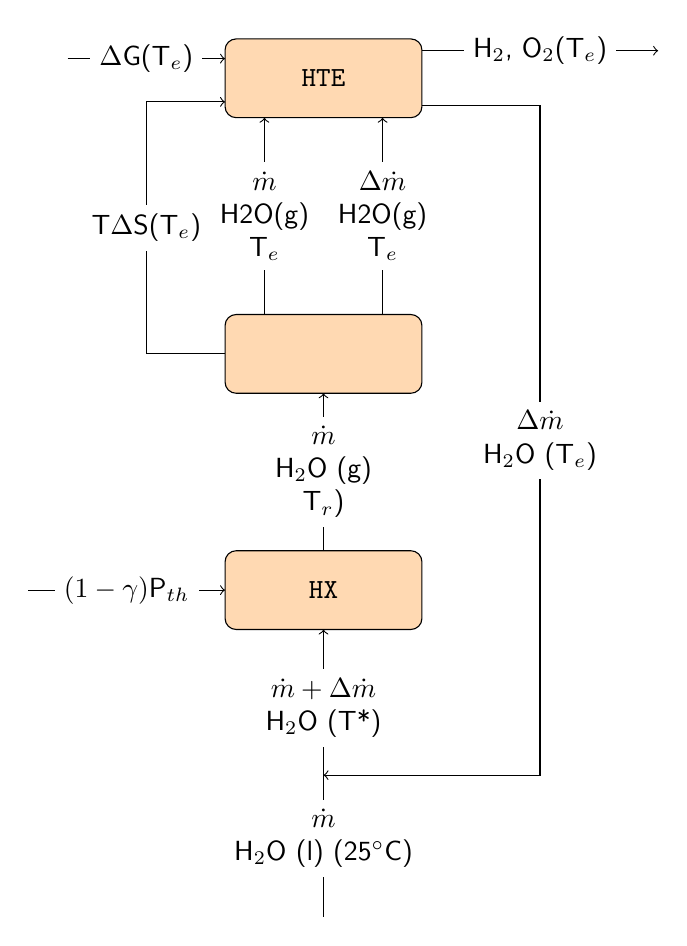
\begin{tikzpicture}[
    base/.style = {rectangle, rounded corners, draw=black,
minimum width=3cm, minimum height=1cm,
text centered, font=\sffamily},
process/.style = {base, minimum width=2.5cm, fill=orange!30,
font=\ttfamily},
node distance=3cm,
every node/.style={fill=white, font=\sffamily}, align=center
]
  % Specification of nodes (position, etc.)

  \node (hte) [process] {HTE};
  \node (split)  [process, below of=hte, yshift=-.5cm] {};
  \node (heat)  [process, below of=split, yshift=0cm] {HX};
  
  \draw[->]     (hte) ++(-3.25,0.25)-- ++(2,0) node[midway] {$\Delta$G(T$_e$)};
  \draw[->]     (hte) ++(1.25,0.35)-- ++(3,0) node[midway] {H$_2$, O$_2$(T$_e$)};
  \draw[->]     (hte) ++(1.25,-0.35)-- ++(1.5,0) -- ++(0,-8.5) node[midway] {$\Delta \dot{m}$\\H$_2$O (T$_e$)} -- ++(-2.75,0);
  \draw[->]     (split) ++(-.75,0.5)-- ++(0,2.5) node[midway] {$\dot{m}$\\H2O(g)\\T$_e$};
  \draw[->]     (split) ++(.75,0.5)-- ++(0,2.5) node[midway] {$\Delta \dot{m}$\\H2O(g)\\T$_e$};
  \draw[->]     (split) ++(-1.25,0) -- ++(-1.,0) -- node[midway] {T$\Delta$S(T$_e$)} ++ (0,3.2) -- ++(1.,0);
  \draw[->]     (split) ++(0,-2.5)-- ++(0,2) node[midway] {$\dot{m}$\\H$_2$O (g)\\T$_r$)};
  \draw[->]     (heat) ++(0,-2.5)-- ++(0,2) node[midway] {$\dot{m}+ \Delta \dot{m}$\\H$_2$O (T*)};
  \draw[-]     (heat) ++(0,-4.15)-- ++(0,2) node[midway] {$\dot{m}$\\H$_2$O (l) (25$^\circ$C)};

  \draw[->]     (heat) ++(-3.75,0)-- ++(2.5,0) node[midway] {$(1-\gamma)$P$_{th}$};

\end{tikzpicture}
}

\end{document}

% To compile do make; make -f hte1.makefile